\chapter{Design of User Interface}
This chapter focuses on how the User Interface should be designed, and the elements it should contain based on the PACT analysis and requirements. Furthermore the chapter will also discuss prototyping, and which prototypes there will be developed in order to test the web application. The User Interface design will be done in close cooperation with Labelless Media, to ensure that the User Interface lives up to their expectations. 
\newline\newline
\noindent
In the development process of the system a course on Udemy is used to help with the setup of both the database, API and front-end since none of the participants in the project have previous expertise with web application development. The key elements used from the course is both the API and front-end programming structure, and the encryption methods which handles login events. INSERT SOURCE TO UDEMY COURSE.

\section{Criteria}
From the meetings with Labelless Media, various criterion for the User Interface have been mentioned. According to Labelless Media, it is important that the User Interface is dummy proof and easy to use and understand. The owner of the company emphasizes that there should be minimal training in how the program should be used. Following the PACT analysis it has also been mentioned that the users of the system has limited IT knowledge and that that the main purpose of upgrading their system, is to simplify and improve the way they are handling their leads. 
\newline \newline
\noindent
The sales personnel is currently working in a competitive environment at Labelless Media. The sales personnel is paid by a commissions based system. According to the owner of Labelless Media it is therefore important that the User Interface is showing how well the sales personnel is performing to improve their motivation. In future plans, Labelless Media wants to focus on subscription based sales. This is, when a Labelless Media and a company agrees on monthly work for a negotiated price over a given time period. This way Labelless Media ensures monthly income and it is thereby easier to hire sales personnel. In order to fulfill Labelless Medias vision of subscription based sales, it is important that the User Interface gives a clear overview of the subscriptions, and is able to manage them.

\section{Display of information}

To examine how the User Interface should be designed, Jakob Nielsen's heuristics about user interface is used. These are ten heuristics that give a general principle of how to create interaction design. This list of principles are called heuristics, because they are not meant to be a specific guideline, but rather used as rules of thumb. Nielsen's ten heuristics are as follows: https://www.nngroup.com/articles/ten-usability-heuristics/
\begin{itemize}
    \item Visibility of system status
    \item Match between system and the real world
    \item User control and freedom
    \item Consistency and standards
    \item Error prevention
    \item Recognition rather than recall
    \item Flexibility and efficiency of use
    \item Aesthetic and minimalist design
    \item Help users recognize, diagnose, and recover from errors
    \item Help and documentation
\end{itemize}
Upon examining the list, some heuristics have been found more relevant than others in relation to this system. These will now be further examined and described.

\subsection{Visibility of system status}
Whenever a change is made in the user interface, the system should give a feedback to the user in form of dialogue boxes. For example when a user edits a lead or creates a comment, the system should tell the user that the lead has been updated, if the event is executed successfully. This way the user should feel comfortable about the changes he or she is making and be ensured that these are updated in the system.

\subsection{Match between system and the real world}
Following the PACT analysis, the users of the system has a limited IT knowledge. It is therefore important that the system speak the users' language. Phrases and concepts used in the system should be identical to the ones the users use in real world conventions. This way, the information in the user interface appears in a natural and logical order, making the user interface intuitive. 

\subsection{Consistency and standards}
To amplify the intuitiveness of the user interface it should contain consistency and standards. Words should be the same throughout the user interface, and components displayed on the user interface will be color coded to match the information state. 

\subsection{Error prevention}
To prevent errors and unsaved changes the user interface should be designed in a way so the users cannot leave states where changes have not been saved. In order to do this, dialogue boxes should be implemented, telling the user that the changes has not been saved yet. Giving the user options to leave the state or to save the changes. 

\subsection{Recognition rather than recall}
To fulfill the criteria of the user interface being intuitive, the user interface will be designed following the recognition rather than recall heuristic by It should be easy to navigate through the system, and the locations of given pages should be intuitive. A location path should be given, in order to tell the user where in the system he or she is currently located. Colors will also be used in order to make the navigation easier and increase readability of the user interface.

\subsection{Aesthetic and minimalist design}
To make the use of the system efficient and understandable only a part of information regarding specific components will be displayed initially. More detailed information about those components will be accessible by double clicking, opening navigation bars, etc. This way, overloading of information is avoided, and aims to increase productivity of the sales personnel. 

\section{Prototypes}
During development of a user interface, prototypes is introduced in order to achieve insight in how real users actually use the product. Two different branches of prototypes are lo-fi and hi-fi prototypes.
\newline \newline
\noindent
Lo-fi prototypes are low tech concepts where the goals is to turn ideas into testable artifacts. Hi-fi prototypes are highly functional and interactive, where the goals is to test usability of the system KILDE:[https://invisionapp.com/inside-design/low-fi-vs-hi-fi-prototyping/]. 
\newline \newline
\noindent
Initially in the development of the user interface a mock-up sketch was drawn in Balsamiq Wireframing tool, to give Labelless Media a general idea of how the user interface could look like. This part of the mock-up is shown in Figure \ref{fig:initialMockup}. The rest of the mock-up is shown in Appendix XXX.
\newline
\begin{figure}[H]
    \centering
    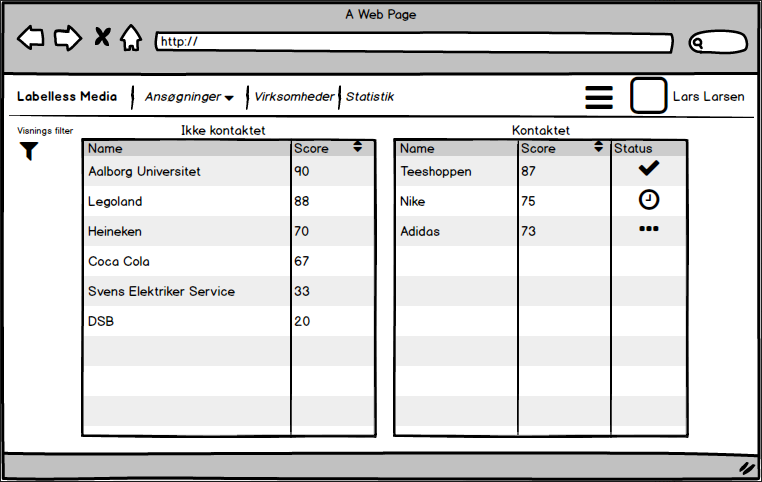
\includegraphics[scale=0.7, clip]{figures/initialMockup.png}
    \caption{The initial mock-up of the system}
    \label{fig:initialMockup}
\end{figure}
\noindent
After discussing the mock-up with Labelless Media, the general layout of the user interface is specified. After the presentation of the mock-up, the owner of Labelless Media had comments on improving the design to match his needs. These c additional tables to categorize leads by their status, and additional super user functionality regarding user handling. 







The owner of Labelless Media was also interested in a hi-fi prototype, or a lo-fi prototype he could interact with. He felt that this was needed, in order for him to give a better review of the design. To fulfill his request, an updated, more detailed lo-fi prototype was again created in Balsamiq Wireframing, this time using their built in interactive feature. This allows linking buttons to specific mock-up pages. 

\section{Summary}
In this chapter several cr